\section{The Evolving Domain Problem}\label{sec:conditional_mixing}

From \S\ref{sec:config-choices}, \base assumes a fixed domain set $\D$. Here, we study the \emph{evolving domain problem} encountered throughout LM development.
We first formalize the problem of recomputing mixes after the domain set is updated (\S\ref{sec:problem-setup-evolving-domain}). We then present \fullmixreuse, our primary mechanism that reuses ratios on all the domains unaffected by the update (\S\ref{sec:mix_reuse_42}). We theoretically analyze when \fullmixreuse performs well (\S\ref{sec:analysis}). Finally, we introduce \partialmixreuse as an extension that reuses the ratios over some unaffected domains (\S\ref{sec:partial-reuse}). An overview of these strategies is provided in Figure~\ref{fig:mixreuse}.

\subsection{Problem Setup}
\label{sec:problem-setup-evolving-domain}

During LM development, the domain set evolves from $\D$ to an updated set $\D' = \{D_1', \dots, D_{m'}'\}$ of size $m'$, where each domain $D_i'$ now has $N_i'$ tokens. We use $q \in \triangle^{m'-1}$ to express data mixtures over $\D'$.
In practice, domain updates are typically localized, affecting only a subset of domains while leaving others unchanged.
To capture this structure, we partition the domain sets as $\D = [\D_1, \D_2]$ and $\D' = [\D_1, \D_2']$, where $\D_1$ is the \textbf{unaffected domain set}, and $\D_2$ is the \textbf{affected domain set} that is transformed into $\D_2'$.

In developing Olmo 1--3~\citep{olmo2025olmo3} and observing similar efforts like SmolLM 1--3~\citep{bakouch2025smollm3}, we identified four patterns of domain updates, which we call \textbf{domain update operators}, that describe how $\D_2$
transforms into $\D_2'$ (Figure~\ref{fig:banner}):
\begin{itemize}
    \item \Add: $\D_2 = \emptyset$ and $\D_2'$ contains the newly added domains. This occurs when new datasets are created.
    \item \Remove: $\D_2$ contains one or more domains and $\D_2' = \emptyset$. This can occur, for instance, when domains are discarded due to low utility.
    \item \Partition: $\D_2$ consists of one domain that is split into multiple subdomains in $\D_2'$ such that $\D_2 = \bigcup_{D_i' \in \D_2'} D_i'$. Partitioning is commonly used to obtain finer-grained mixtures, which can improve performance~\citep{wettig2025organizewebconstructingdomains, diao2025climbclusteringbasediterativedata,ge2025rbdomainregroupingdata, peng2025topicsourcekeyeffective}.
    \item \Revise: $\D_2$ is one domain that is modified to produce the corresponding domain in $\D_2'$. This occurs when contents of the dataset are modified, such as samples being reformatted or rewritten~\citep{kimiteam2025kimik2openagentic, maini2024rephrasingwebrecipecompute}.
\end{itemize}

\textbf{Goal.} We have an existing mixture $\tilde{p} \in \triangle^{m-1}$ over the current domain set $\D$ proposed through a procedure like \base. 
But now, the domain set has evolved from $\D$ to $\D'$, and our goal is to use $\tilde{p}$ to compute an updated optimal $q^\star \in \triangle^{m' - 1}$ on $\D'$ that solves
\begin{align}
    &\text{minimize}_{q \in \triangle^{m'-1}}  \frac{1}{n} \sum_{i = 1}^n f_i(\LM(S, R, q))
    \label{eq:mixing_problem} \\
    &\text{s.t.} \quad  q_j \le \frac{k N_j'}{R} \quad \forall j \in [m'] \nonumber
\end{align}

This objective is similar to the one in \S\ref{sec:setup_1}, except that it is defined over $q$, and we explicitly enforce the repetition constraint from \S\ref{sec:optimization} to ensure that samples are not repeated more than $k$ times.

\textbf{Baseline: full recomputation.} One way to solve~\eqref{eq:mixing_problem} is to apply \base (Algorithm~\ref{alg:base_method}) to $\D'$ after each update, which requires a swarm of $\mathcal{O}(m')$ proxy runs (\S\ref{sec:swarm}). The costs of full recomputation thus accumulate rapidly with the number of updates. We next study whether mixture reuse can produce mixes at a lower cost.

\subsection{Mixture Reuse}\label{sec:mix_reuse_42}

The core idea in mixture reuse is to freeze the relative ratios among the unaffected domains according to $\tilde{p}$, aggregate them into a single \emph{virtual domain}, and only recompute its total weight along with the weights of the affected domains $\mathcal{D}_2'$. This reduces the dimensionality of the optimization from $m'$ to $1 + |\mathcal{D}_2'|$. This mechanism is presented in Figure~\ref{fig:mixreuse} (right).

For example, suppose $\mathcal{D}$ contains $m=3$ domains with mixture
$\tilde{p} = [0.25,\,0.25,\,0.5]$, and $\mathcal{D}'$ is formed by adding
one new domain.
Instead of learning a $4$-dimensional mixture, we learn a $2$-dimensional
mixture over the virtual domain and the new domain.
If that mixture is $[0.4,\,0.6]$,  we can expand it using $\tilde{p}$ to induce the final mixture over $m'=4$ domains:
\[
q=\underbrace{0.4}_{\substack{\text{recomputed}\\\text{virtual domain}\\\text{ratio}}} \cdot \underbrace{[0.25,\,0.25,\,0.5]}_{\substack{\text{reused}\\\text{ratios}}} \;\cup\; \underbrace{[0.6]}_{\substack{\text{recomputed}\\\text{affected domain}\\\text{ratio}}}\;=\; [0.1,\,0.1,\,0.2,\,0.6].
\]
See Appendix~\ref{supp:examples} for examples of \Remove, \Partition, and \Revise.

\begin{figure}
    \centering
    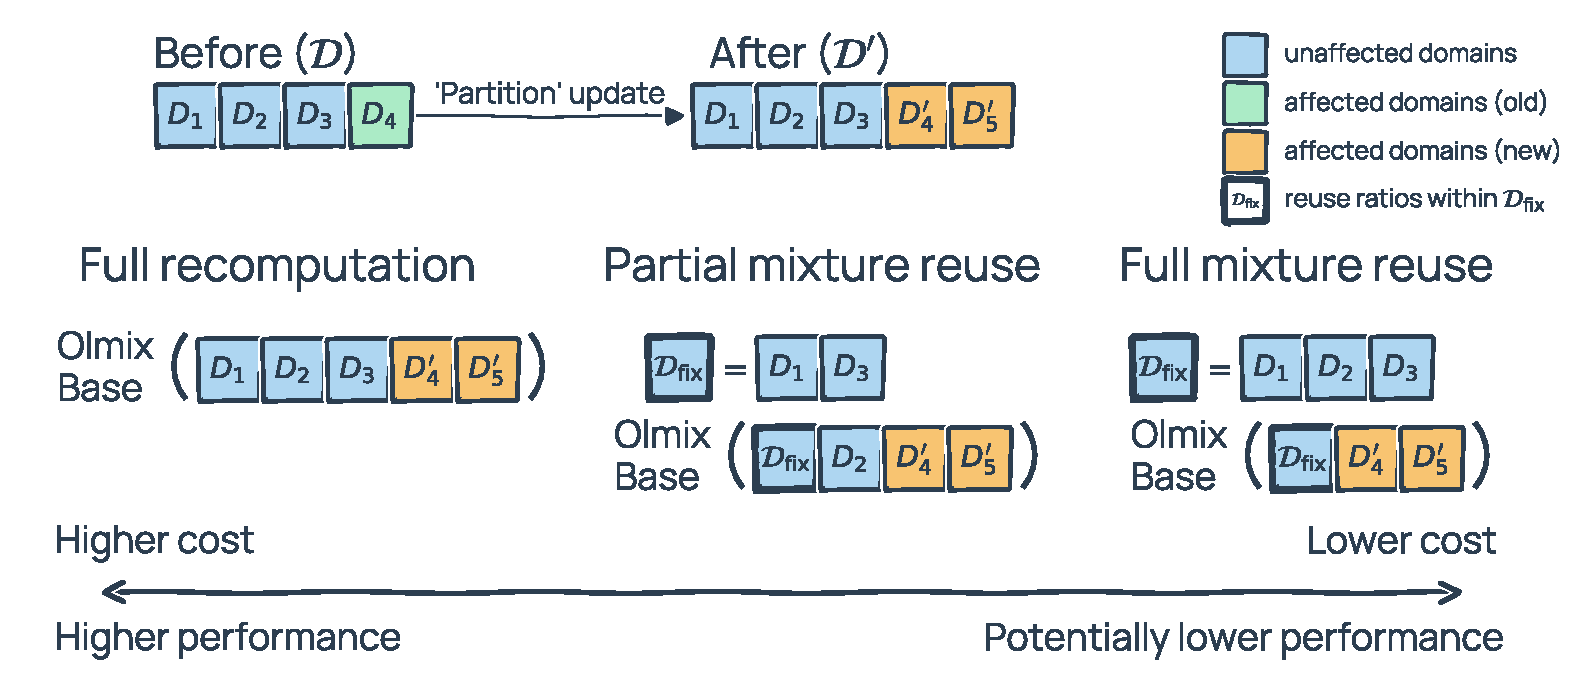
\includegraphics[width=0.8\linewidth]{figs/fig_mixreuse_new.pdf}
    \caption{Overview of Mixture Recomputation Strategies. When the domain set is updated, full recomputation applies \base on the entire $\D'$, while \fullmixreuse (\S\ref{sec:mix_reuse_42}) and \partialmixreuse (\S\ref{sec:partial-reuse}) freeze the ratios of the domains in $\Dfix$, resulting in less recomputation. The strategies provide a spectrum in terms of cost (number of swam runs) and downstream performance.}
    \label{fig:mixreuse}
\end{figure}





\subsubsection{Formalizing the Mixture Reuse Problem}

The example above provides the intuition behind mixture reuse, which we formalize in the mixture reuse problem. First, we introduce notation to handle domains we will reuse versus recompute. Define $\Dfix := \D_1$ as the unaffected domains whose relative ratios we will keep fixed from $\tilde{p}$, and $\Dcomp := \D_2'$ as the affected domains whose ratios we recompute. We remap these domain sets because, as seen later in \S\ref{sec:partial-reuse}, we may choose to recompute unaffected domains.


We partition any mix $q$ on $\D'$ as $q = [\rho q_{\Dfix}, (1 - \rho) q_{\Dcomp}]$, where $\rho \in [0, 1]$ is the total weight on the unaffected domains, and $q_{\Dfix} \in \triangle^{|\Dfix| - 1}$ and $q_{\Dcomp} \in \triangle^{|\Dcomp| - 1}$ are the relative mixes within $\Dfix$ and $\Dcomp$, respectively. 
Similarly, we define $\tilde{p}_{\Dfix} \in \triangle^{|\Dfix| - 1}$ as the normalized ratios from $\tilde{p}$ restricted to $\Dfix$.


With this notation, the mixture reuse problem is the following approximation of~\eqref{eq:mixing_problem}:
\begin{align}
    &\text{minimize}_{q \in \triangle^{m'-1}}  \frac{1}{n} \sum_{i = 1}^n f_i(\LM(S, R, q))
    \label{eq:conditional_mixing_problem} \\
    &\text{s.t.} \quad  q_j \le \frac{k N_j'}{R} \quad \forall j \in [m'] \nonumber \\
    &  \qquad \; \textcolor{olmoBlue}{q_{\Dfix} = \tilde{p}_{\Dfix}} \nonumber 
\end{align}

The new constraint $\textcolor{olmoBlue}{q_{\Dfix} = \tilde{p}_{\Dfix}}$ enforces that the relative ratios among $\Dfix$ are the same as in $\tilde{p}$; we optimize over a simpler $q$ of the form $[\rho \textcolor{olmoBlue}{\tilde{p}_{\Dfix}}, (1 - \rho) q_{\Dcomp}]$.

\subsubsection{\fullmixreuse} 





We now describe \fullmixreuse, our approach for solving the mixture reuse problem~\eqref{eq:conditional_mixing_problem}.


We use a change of variables that absorbs the constraint $q_{\Dfix} = \tilde{p}_{\Dfix}$, transforming~\eqref{eq:conditional_mixing_problem} into an unconstrained optimization problem.
For any feasible $q = [\rho \tilde{p}_{\Dfix}, (1 - \rho) q_{\Dcomp}]$, we aggregate all domains in $\Dfix$ into a single virtual domain and define the collapsed mixture $r = [\rho, (1-\rho)q_{\Dcomp}] \in \triangle^{|\Dcomp|}$. 
We index the elements of $r$ by $\{v\} \cup \Dcomp$, where $r_v = \rho$ denotes the virtual domain weight (the total weight on $\Dfix$) and $r_j$ for $j \in \Dcomp$ are the weights on affected domains.
Given $\tilde{p}_{\Dfix}$, any collapsed mixture $r$ can be expanded into a feasible $q$ over $\D'$ via the expansion function $\Phi_{\tilde{p}_{\Dfix}}(r)$, where $q_j = r_v \cdot \tilde{p}_j$ for $j \in \Dfix$, and $q_j = r_j$ for $j \in \Dcomp$. 


From our earlier example, $r = [0.4, 0.6]$ (i.e., $\rho = 0.4$ and $q_{\Dcomp} = [1]$) with $\tilde{p}_{\Dfix} = [0.25, 0.25, 0.5]$ expands into $q = \Phi_{\tilde{p}_{\Dfix}}(r) = [0.1, 0.1, 0.2, 0.6]$.

This change of variables transforms the mixture reuse problem into standard mixing on $r$ over $1 + |\Dcomp|$ domains (Lemma~\ref{lem:collapsed_space}). We can now apply \base (Algorithm~\ref{alg:base_method}) in the collapsed space, which requires only $\mathcal{O}(|\Dcomp|)$ proxy runs instead of $\mathcal{O}(m')$. 
The result is a proposed collapsed mixture $r^\star(\tilde{p}_{\Dfix})$, which we expand back to the full domain space as $q^\star(\tilde{p}_{\Dfix}) = \Phi_{\tilde{p}_{\Dfix}}(r^\star(\tilde{p}_{\Dfix}))$. This expanded mixture is our final proposed mix over $\D'$. The full procedure is in Algorithm~\ref{alg:conditional_mixing_method}, with \textcolor{olmoBlue}{blue} text indicating changes from \base in Algorithm~\ref{alg:base_method}.


\begin{figure}[htb]
\centering
\begin{tikzpicture}
\node[inner sep=0pt] (alg) {
\begin{minipage}{0.9\textwidth}
\begin{algorithm}[H]
   \caption{\fullmixreuse}
   \label{alg:conditional_mixing_method}
\begin{algorithmic}[1]
   \STATE {\bfseries Input:} \textcolor{olmoBlue}{Domain set $\D' = \Dfix \cup \Dcomp$ of sizes $\{N_1', \dots, N_{m'}' \}$, existing mix $\tilde{p} \in \triangle^{m - 1}$}, swarm size $K = \mathcal{O}(m)$, repetition factor $k$, requested tokens $R$, KL penalty $\lambda$, natural distribution $r_0 \in \triangle^{|\Dcomp|}$.
    \STATE Sample mixes $r^1, \dots, r^K \in \triangle^{|\Dcomp|}$ and \textcolor{olmoBlue}{expand each collapsed mix $r^j$ into $q^j := \Phi_{\tilde{p}_{\Dfix}}(r^j)$}.
    \STATE Train proxy models on the expanded mixes and evaluate on downstream tasks to get a dataset of mixes and performance, $\{(r^j, \{y_{ij}\}_{i = 1}^n \}_{j =1}^K$, where $y_{ij}:= f_i(\LM(\Ssmall, \Rsmall, q^j))$.
    \FOR{$i \in [n]$}
        \STATE Use $\{(r^j, y_{ij})\}_{j = 1}^K$ to fit the log-linear model $\hat{g}_i(r) = d_i + \exp(B_i^\top r)$, where $d_i \in \R^+$ and $B_i \in \R^{|\Dcomp|}$.
    \ENDFOR
    \STATE Solve the following optimization problem to get $r^\star(\tilde{p}_{\Dfix})$:
    \begin{align}
    &\text{minimize}_{r \in \triangle^{|\Dcomp|}} \frac{1}{n} \sum_{i=1}^n \hat{g}_i(r) + \lambda \kl(r || r_0) \label{eq:alg_mixing_problem_2} \nonumber \\ & \text{subject to} \quad r_v \leq \min_{j \in \Dfix}\bigg\{\frac{k N_j'}{R \tilde{p}_{j}} \bigg\}, \;\; r_j \le  \frac{k N_j'}{R} \quad \forall j \in \Dcomp \nonumber 
    \end{align}
   \STATE \textbf{Return} \textcolor{olmoBlue}{$q^\star(\tilde{p}_{\Dfix}) := \Phi_{\tilde{p}_{\Dfix}}(r^\star(\tilde{p}_{\Dfix}))$, the expanded form of $r^\star(\tilde{p}_{\Dfix})$}.
\end{algorithmic}
\end{algorithm}
\end{minipage}
};

\draw [decorate,decoration={brace,amplitude=5pt}]
    ([yshift=-2.5cm,xshift=5pt]alg.north east) -- ([yshift=-3.8cm,xshift=5pt]alg.north east)
    node[midway,right=10pt,rotate=-90,anchor=south] {\footnotesize Swarm};
    
\draw [decorate,decoration={brace,amplitude=5pt}]
    ([yshift=-3.9cm,xshift=5pt]alg.north east) -- ([yshift=-5.4cm,xshift=5pt]alg.north east)
    node[midway,right=8pt,rotate=-90,anchor=south] {\footnotesize Regression};
    
\draw [decorate,decoration={brace,amplitude=5pt}]
    ([yshift=-5.5cm,xshift=5pt]alg.north east) -- ([yshift=-8.5cm,xshift=5pt]alg.north east)
    node[midway,right=8pt,rotate=-90,anchor=south] {\footnotesize Optimization};
\end{tikzpicture}
\end{figure}




\subsection{Theoretical Analysis}\label{sec:analysis}

\fullmixreuse reduces costs by reusing existing ratios, but when does it match versus degrade performance compared to full recomputation? We theoretically analyze this, finding that performance depends on (1) how much the optimal mix changes due to the domain update, and (2) a coupling effect between $\Dfix$ and $\Dcomp$.
Importantly, we empirically validate our theory in \S\ref{sec:validation}: \textbf{we measure the terms in our bounds and show they tightly track actual performance gaps across settings.}

\textbf{Assumptions.} We make the following assumptions.
\begin{enumerate}[itemsep=0pt,topsep=2pt,leftmargin=12pt]
    \item Log linear model holds: For each task $i\in[n]$, performance can be expressed as $f_i(\LM(S,R,q)) = c_i + \exp(A_i^\top q)$ for some $c_i\in\R^+,\; A_i\in\R^{m'}$.
    \item Full recomputation minimizes~\eqref{eq:mixing_problem}, and \fullmixreuse minimizes~\eqref{eq:conditional_mixing_problem}. 
\end{enumerate}


\textbf{Definitions.}
Define performance of $q$ as $F(q) := \frac{1}{n}\sum_{i=1}^n f_i(\LM(S,R,q))$. $q^\star$ is the solution to~\eqref{eq:mixing_problem}, and $q^\star(\tilde p_{\Dfix})$ is the solution to~\eqref{eq:conditional_mixing_problem}. We study the \emph{performance gap} of \fullmixreuse, $F(q^\star(\tilde p_{\Dfix})) \texttt{-} F(q^\star)$.

Let $q^\star_{\Dfix}$ denote the optimal mix on $\Dfix$ after the domain set update, such that $q^\star = [\rho^\star q^\star_{\Dfix},\; (1-\rho^\star)q^\star_{\Dcomp}]$. Let $\kappa(\Dfix, \Dcomp)$ denote a coupling term (defined in Appendix~\ref{supp:defs}) that captures task influence of $\Dfix$ versus $\Dcomp$.



\subsubsection{Performance Characterization}

Our first result characterizes the performance gap in terms of $\tilde{p}_{\Dfix}$ itself. See Appendix~\ref{supp:general_gap_proof} for the proof. 


\begin{theorem}[Performance gap bound] \label{thm:general_gap} There exists a finite $C_1 > 0$ such that the performance gap is bounded by
\begin{align*} 
&F(q^\star(\tilde{p}_{\Dfix})) - F(q^\star) \le C_1 \kappa(\Dfix, \Dcomp) \|\tilde{p}_{\Dfix} - q^\star_{\Dfix}\|.
\end{align*} 
\end{theorem}


The performance gap is controlled by two factors: \begin{itemize}[itemsep=0pt,topsep=2pt,leftmargin=12pt] 
\item $\|\tilde{p}_{\Dfix} - q^\star_{\Dfix} \|$ (``reuse gap''): how close the mix we reuse is to the optimal mix after the update. 
\item $\kappa(\Dfix, \Dcomp)$: this coupling term is large when $\Dfix$ and $\Dcomp$ impact the same set of downstream tasks. It controls the rate at which performance depends on the reuse gap. 
\end{itemize}


When both terms are small, \fullmixreuse matches full recomputation. Our empirical validation (Figure~\ref{fig:theorem1_validation}) confirms that the reuse gap strongly predicts actual performance gaps across different scenarios.


\subsubsection{Reuse Gap}

Theorem~\ref{thm:general_gap} shows that the performance gap is governed by the reuse gap, but when is the reuse gap small? 
We analyze the case where $\tilde{p}$ is assumed to be optimal before the update, and the domain set is modified via an \Add update.
Proofs and results on other operators are in Appendix~\ref{supp:add_domains_proof}.



\begin{theorem}\label{thm:add_domains}
Define $\tilde{p}$ as the solution to~\eqref{eq:mixing_problem} on $\D$ and suppose that new domains are added. There exists a finite $C_2 > 0$ such that the reuse gap is bounded by
    \begin{align*}
        \|\tilde{p}_{\Dfix} - q^\star_{\Dfix}\| \le C_2 \kappa(\Dfix, \Dcomp) (1 - \rho^\star).
    \end{align*}
\end{theorem}

The reuse gap is controlled by two factors:
\begin{itemize}[itemsep=0pt,topsep=2pt,leftmargin=12pt]
    \item $\kappa(\Dfix, \Dcomp)$: the coupling term, also in Theorem~\ref{thm:general_gap}.
    \item $1 - \rho^\star$: this term captures how much newly added domains move the optimum, since $1$ is effectively $\rho$ induced by $\tilde{p}$ before domains are added. This term can be small when: 1) the added domains are low utility, or 2) the added domains have little data, so the repetition constraint caps their maximum weight.
\end{itemize}    

Our empirical validation (Figures \ref{fig:theorem2_validation}- \ref{fig:theorem2_validation_coupling}) shows that the success of \fullmixreuse when adding domains correlates with small $1-\rho^\star$ and low coupling.


\subsection{\partialmixreuse}
\label{sec:partial-reuse}

Our analysis (\S\ref{sec:analysis}) shows that \fullmixreuse may underperform full recomputation when coupling between $\Dfix$ and $\Dcomp$ is high. We propose \partialmixreuse (Figure~\ref{fig:mixreuse} center) as a middle ground: rather than reusing all unaffected domains, it selectively recomputes some, reducing coupling while keeping costs below full recomputation.


\textbf{Method} Let $\Dpartial \subset \D_1$ be a subset of unaffected domains we reuse. We redefine the domains we reuse versus recompute as $\Dfix := \Dpartial$ and $\Dcomp := (\D_1 \setminus \Dpartial) \cup \D_2'$, and then apply \fullmixreuse (Algorithm~\ref{alg:conditional_mixing_method}) with this new partition. The mixing problem has dimension $1 + |\D_2'| + |\D_1 \setminus \Dpartial|$, interpolating between \fullmixreuse's $1 + |\D_2'|$ and full recomputation's $m'$. Since swarm cost scales linearly with dimension (RQ2), this directly interpolates computational cost.

\textbf{Interpretation and Empirical Validation} Carefully choosing $\Dpartial$ can reduce the coupling $\kappa(\Dfix, \Dcomp)$ from Theorem~\ref{thm:general_gap}. 
An intuitive example: when adding code data to web topics, the software development web topic should be recomputed alongside it since both strongly influence code evaluation tasks. Figure~\ref{fig:theorem2_validation_coupling} confirms that this reduces coupling and improves performance compared to reusing all web topics.
